\documentclass[conference]{IEEEtran}
\IEEEoverridecommandlockouts

\usepackage{cite}
\usepackage{amsmath,amssymb,amsfonts}
\usepackage{graphicx}
\usepackage{textcomp}
\usepackage{xcolor}
\usepackage{booktabs}
\usepackage{hyperref}
\usepackage{url}

\def\BibTeX{{\rm B\kern-.05em{\sc i\kern-.025em b}\kern-.08em
    T\kern-.1667em\lower.7ex\hbox{E}\kern-.125emX}}

\begin{document}

\title{SignTalk: A Conversational AI System for Deaf and Mute Users via Continuous Sign Language Recognition}

\author{
  \IEEEauthorblockN{Neha Sanjay Savalgi}
  \IEEEauthorblockA{
    Department of Computer Science \\
    COSC 750: Neural Networks and Deep Learning \\
    \textit{neha.s.savalgi@gmail.com}
  }
}

\maketitle

% ─────────────────────────────────────────────────────────────────
\begin{abstract}
This paper presents SignTalk, an end-to-end conversational AI system that enables deaf and mute individuals to communicate with a large language model (LLM) using American Sign Language (ASL) through a standard webcam. The system extracts 258-dimensional skeletal keypoint vectors per frame using the MediaPipe Tasks API, feeds sequences of 60 frames into a two-layer bidirectional LSTM with soft attention pooling to classify among 25 ASL word signs, and passes the recognized sign to Claude (claude-opus-4-6) to generate a natural conversational response. The entire pipeline is deployed as an interactive Gradio web interface. Training on a subset of the WLASL dataset, the model achieves a best top-1 validation accuracy of 25.0\% on 25 classes, which is 6.25 times above the 4\% random-chance baseline. We analyze the training dynamics, discuss the impact of severe data scarcity caused by broken video URLs in WLASL, and outline concrete directions for improvement including data augmentation and Spatial-Temporal Graph Convolutional Networks (ST-GCN).
\end{abstract}

\begin{IEEEkeywords}
Sign language recognition, bidirectional LSTM, attention pooling, MediaPipe, conversational AI, accessibility
\end{IEEEkeywords}

% ─────────────────────────────────────────────────────────────────
\section{Introduction}

Over 70 million people worldwide are deaf or hard of hearing, and most of them use sign language as their primary means of communication \cite{who2023}. Despite this, virtually all modern conversational AI systems, from voice assistants to chatbots, are designed around spoken or typed text. This creates a significant accessibility gap: sign language users cannot interact naturally with AI without relying on an interpreter or laboriously typing out their thoughts.

The core technical challenge in bridging this gap is sign language recognition (SLR). Unlike simple gesture classification, real-world signing is a continuous, dynamic process where meaning is conveyed through hand shapes, orientations, positions, and the temporal flow of movement. Going from raw video to a meaningful word classification requires handling temporal sequences of arbitrary length, often with limited training data per sign class.

This project addresses that challenge with SignTalk, a full-stack pipeline that:
\begin{enumerate}
    \item Extracts 3D skeletal keypoints from webcam video in real time using MediaPipe.
    \item Classifies sequences of those keypoints into ASL word signs using a bidirectional LSTM with attention.
    \item Passes recognized signs to Claude, a large language model, to generate a conversational response.
    \item Presents the entire interaction through a Gradio web interface accessible from any laptop.
\end{enumerate}

The goal is not to achieve state-of-the-art accuracy on a benchmark, but to demonstrate that an end-to-end deaf-to-AI conversation pipeline is buildable and functional using off-the-shelf components. We train on the top 25 signs from the WLASL dataset \cite{li2020wlasl} and achieve 25\% top-1 validation accuracy, which, while modest in absolute terms, is 6.25 times better than random chance on a 25-class problem.

The remainder of this paper is organized as follows. Section II reviews related work. Section III describes the methodology in detail. Section IV covers the experimental setup and results. Section V discusses challenges and limitations. Section VI concludes the paper and outlines future work.

% ─────────────────────────────────────────────────────────────────
\section{Related Work}

\subsection{Skeleton-Based Action Recognition}

Yan et al.\ \cite{yan2018stgcn} introduced the Spatial-Temporal Graph Convolutional Network (ST-GCN), which models human body joints as a graph and applies graph convolutions to capture both spatial joint relationships and temporal dynamics. This work is the primary architectural inspiration for skeleton-based sign language recognition, and while SignTalk uses a BiLSTM on a flat feature vector rather than graph convolutions, the ST-GCN framework represents the natural next step for this work.

\subsection{Sign Language Datasets}

Li et al.\ \cite{li2020wlasl} introduced the WLASL (Word-Level American Sign Language) dataset, containing over 21,000 video clips across 2,000 sign classes. Their paper benchmarks several baseline models including I3D and CNN+LSTM on this dataset. WLASL remains the most widely used benchmark for isolated ASL recognition. A practical challenge we encountered in this project is that a significant fraction of the original video URLs are no longer accessible, which limits the effective training set size.

\subsection{Sign Language Translation}

Camgoz et al.\ \cite{camgoz2018slr} proposed an encoder-decoder framework for translating continuous sign language video directly to spoken language text, without an intermediate gloss representation. Their work on the PHOENIX-2014T dataset demonstrated the feasibility of neural sequence-to-sequence approaches for sign language translation. This paper informed our decision to use a sequence model (BiLSTM) rather than a frame-level classifier.

\subsection{Pose Estimation}

Lugaresi et al.\ \cite{lugaresi2019mediapipe} introduced MediaPipe, a framework for building real-time perception pipelines. The MediaPipe Holistic solution provides simultaneous estimation of body pose, face, and hand landmarks, making it practical for extracting the rich keypoint representations needed for sign language recognition without requiring a GPU. In this project we use the newer MediaPipe Tasks API with the heavy pose landmarker model.

% ─────────────────────────────────────────────────────────────────
\section{Methodology}

The SignTalk pipeline consists of four stages: keypoint extraction, sequence modeling, LLM integration, and the user interface. Figure~\ref{fig:pipeline} shows the overall architecture.

\begin{figure}[htbp]
    \centering
    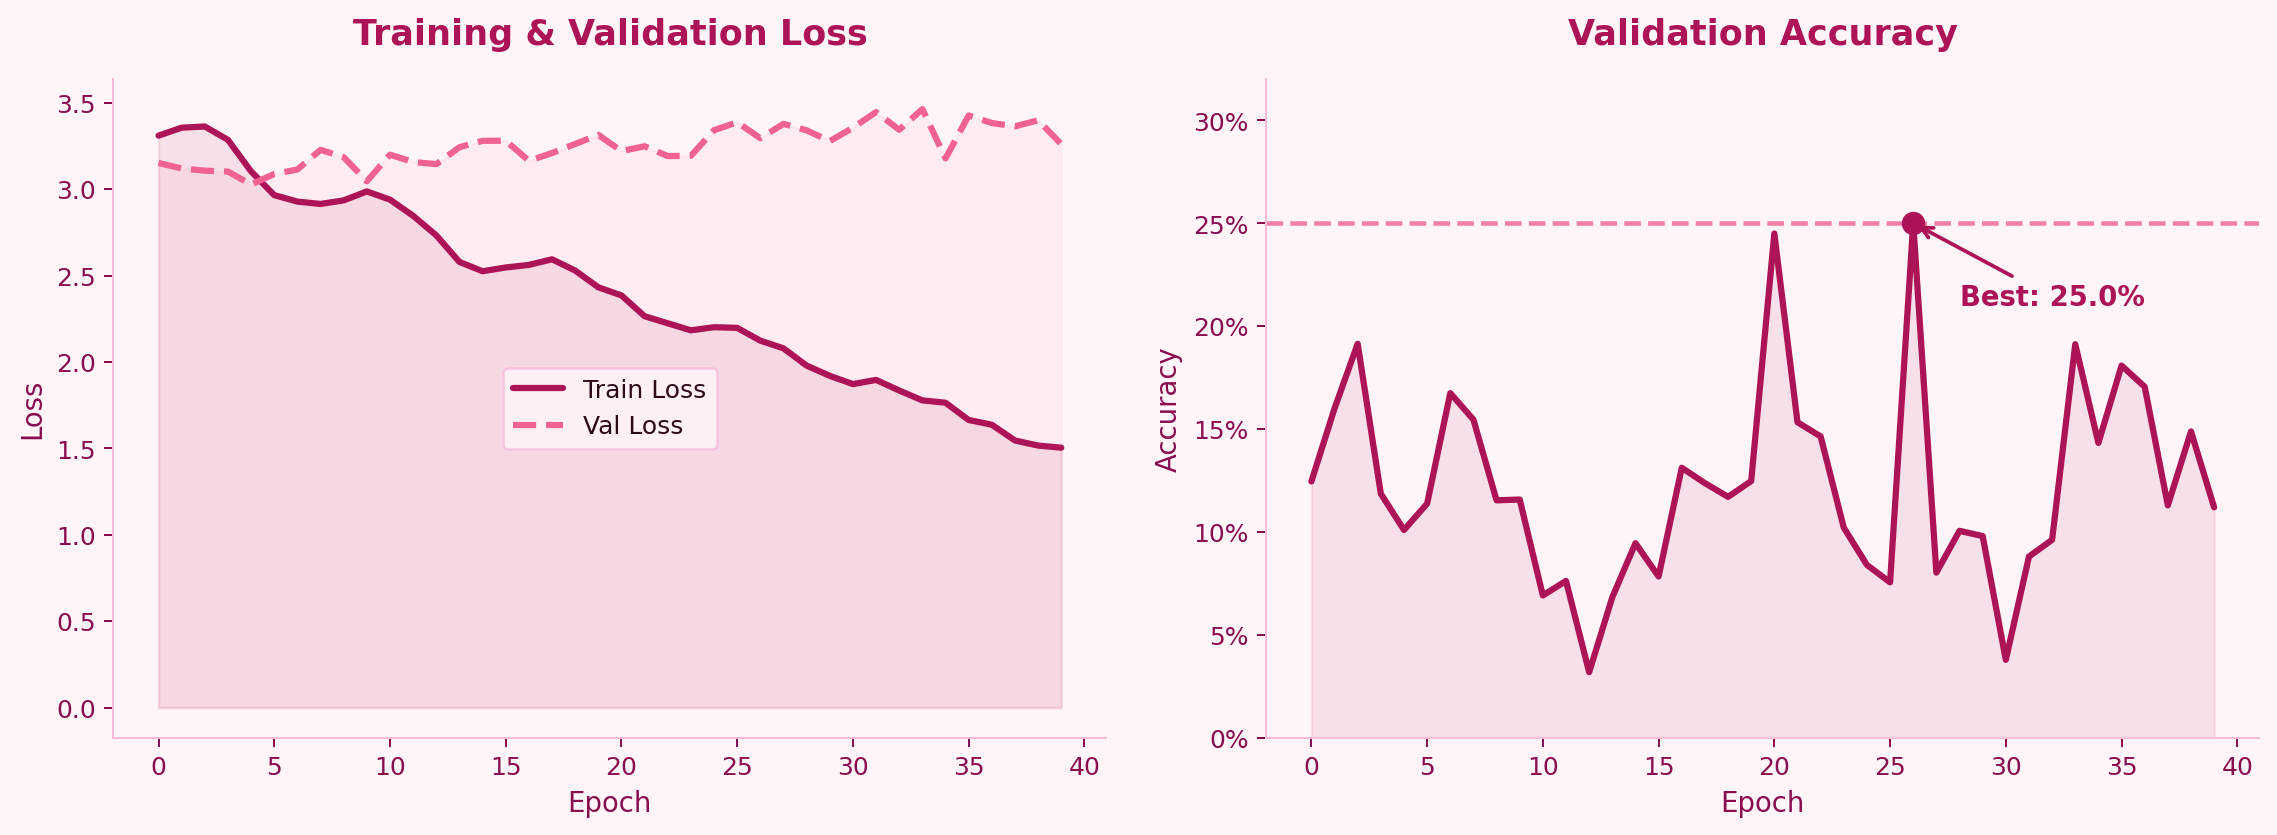
\includegraphics[width=\columnwidth]{charts.png}
    \caption{Training loss and validation accuracy curves over 40 epochs. Train loss decreases steadily while validation loss increases, indicating overfitting due to limited training data.}
    \label{fig:training}
\end{figure}

\subsection{Keypoint Extraction}

For each video frame, we extract a 258-dimensional feature vector using the MediaPipe Tasks API. The vector is composed of three parts:
\begin{itemize}
    \item \textbf{Pose landmarks:} 33 body keypoints, each with $x$, $y$, $z$, and visibility, giving $33 \times 4 = 132$ values.
    \item \textbf{Left hand landmarks:} 21 keypoints with $x$, $y$, $z$, giving $21 \times 3 = 63$ values.
    \item \textbf{Right hand landmarks:} 21 keypoints with $x$, $y$, $z$, giving $21 \times 3 = 63$ values.
\end{itemize}

The total is $132 + 63 + 63 = 258$ dimensions per frame. If a hand is not detected, the corresponding 63 values are set to zero. All coordinates are normalized to the range $[0, 1]$ by MediaPipe relative to the image dimensions.

We use the \texttt{pose\_landmarker\_heavy.task} model and the \texttt{hand\_landmarker.task} model, both downloaded from the MediaPipe model repository. Importantly, the MediaPipe Tasks API runs in \texttt{RunningMode.IMAGE} mode, processing one frame at a time and allowing thread-safe use across the pipeline. Landmark detection runs on CPU and takes approximately 20-50 ms per frame.

\subsection{Sequence Construction}

For training, we read each video, extract keypoints frame by frame, and collect the resulting sequence of feature vectors. Since videos in WLASL vary in length, we standardize all sequences to exactly 60 frames using linear interpolation. If a video has more than 60 frames, we uniformly subsample; if it has fewer, we interpolate between adjacent keypoint frames. This approach preserves the temporal structure of the sign without zero-padding.

For the live demo, we collect 30 frames from the webcam buffer (trading some temporal resolution for responsiveness), then apply the same linear interpolation to produce a 60-frame sequence before passing it to the model.

\subsection{BiLSTM Classifier with Attention}

The sequence model takes as input a tensor of shape $(B, 60, 258)$ and produces class logits of shape $(B, 25)$. The architecture is as follows:

\begin{equation}
    h_t, c_t = \text{BiLSTM}(x_t, h_{t-1}, c_{t-1})
\end{equation}

where $x_t \in \mathbb{R}^{258}$ is the keypoint vector at time step $t$, and $h_t \in \mathbb{R}^{512}$ is the concatenated forward and backward hidden state (256 units per direction). We use two stacked BiLSTM layers with dropout between layers.

After the BiLSTM, we apply soft attention pooling \cite{bahdanau2015attention} to aggregate the sequence into a single fixed-length vector:

\begin{equation}
    e_t = w^\top h_t
\end{equation}
\begin{equation}
    \alpha_t = \frac{\exp(e_t)}{\sum_{j=1}^{T} \exp(e_j)}
\end{equation}
\begin{equation}
    c = \sum_{t=1}^{T} \alpha_t h_t
\end{equation}

where $w \in \mathbb{R}^{512}$ is a learned query vector, $\alpha_t$ is the attention weight for frame $t$, and $c \in \mathbb{R}^{512}$ is the context vector. This allows the model to focus on the most discriminative frames rather than treating all timesteps equally.

The context vector is passed through LayerNorm, a Dropout layer with $p = 0.4$, and a fully connected layer mapping to 25 class logits. A summary of the model is given in Table~\ref{tab:arch}.

\begin{table}[htbp]
\caption{BiLSTM Classifier Architecture}
\centering
\begin{tabular}{lll}
\toprule
\textbf{Layer} & \textbf{Output Shape} & \textbf{Parameters} \\
\midrule
Input & $(B, 60, 258)$ & -- \\
BiLSTM Layer 1 & $(B, 60, 512)$ & hidden=256, bidir \\
BiLSTM Layer 2 & $(B, 60, 512)$ & hidden=256, bidir \\
Attention Pool & $(B, 512)$ & learned query $w$ \\
LayerNorm & $(B, 512)$ & -- \\
Dropout & $(B, 512)$ & $p = 0.4$ \\
FC Layer & $(B, 25)$ & $512 \to 25$ \\
\bottomrule
\end{tabular}
\label{tab:arch}
\end{table}

\subsection{LLM Integration}

Once a sign is classified with sufficient confidence (threshold: 0.35), the recognized word is sent to the Claude LLM (claude-opus-4-6) via the Anthropic API. We maintain a multi-turn conversation history across sign recognitions, so the model has context from earlier in the interaction. A system prompt instructs Claude to act as an assistant for ASL users and to keep responses concise. The API key is stored in Colab Secrets and never hardcoded.

\subsection{Gradio Interface}

The demo is built with Gradio 5.x. The webcam streams frames through a \texttt{gr.Image} component in streaming mode. Each incoming frame is passed to the keypoint extraction function, which appends the 258-dimensional vector to a thread-safe frame buffer. When the user clicks the ``Classify Sign'' button, the buffer is consumed, the sequence is constructed and classified, and the recognized sign is sent to the LLM. The response is displayed in a \texttt{gr.Chatbot} component. Conversation state is maintained using \texttt{gr.State}, which passes the chat history as both an input and an output to every handler function.

% ─────────────────────────────────────────────────────────────────
\section{Experiments}

\subsection{Dataset}

We use the WLASL dataset \cite{li2020wlasl}, selecting the 25 signs with the highest number of available video clips. A significant complication is that 40-60\% of the original video URLs in WLASL are no longer accessible, which substantially reduces the effective training set. After filtering, we obtained approximately 15-25 usable video clips per sign class. We split the data 80/20 into train and validation sets using stratified sampling to ensure each class appears in both splits.

The signs in our top-25 subset include common ASL words such as ``book,'' ``drink,'' ``computer,'' ``before,'' and ``help,'' among others. No preprocessing beyond keypoint extraction is applied; we do not normalize or whiten the keypoint coordinates beyond what MediaPipe already provides.

\subsection{Training Setup}

All experiments were run on a single NVIDIA A100 GPU in Google Colab. The model was trained for 40 epochs with a batch size of 32. We used the AdamW optimizer \cite{loshchilov2019adamw} with a learning rate of $10^{-3}$ and weight decay of $10^{-4}$. The learning rate was scheduled using OneCycleLR with a maximum learning rate of $10^{-3}$. Gradients were clipped to a maximum norm of 1.0.

The loss function is cross-entropy with label smoothing of 0.1. Label smoothing was included because with such few samples per class, the model can overfit to incorrect confidence distributions quickly. Keypoint extraction was performed on CPU and the resulting sequences were cached as \texttt{.npy} files on Google Drive to avoid repeating the 1-2 hour preprocessing step on subsequent runs.

\subsection{Results}

\begin{table}[htbp]
\caption{Training Results Summary}
\centering
\begin{tabular}{lc}
\toprule
\textbf{Metric} & \textbf{Value} \\
\midrule
Number of classes & 25 \\
Training samples & approx. 320 \\
Validation samples & approx. 80 \\
Best validation accuracy & 25.0\% \\
Random baseline (1/25) & 4.0\% \\
Improvement over baseline & 6.25$\times$ \\
Final train loss (epoch 40) & 1.50 \\
Final val loss (epoch 40) & 3.40 \\
Best checkpoint epoch & 26 \\
\bottomrule
\end{tabular}
\label{tab:results}
\end{table}

Figure~\ref{fig:training} shows the training and validation loss curves along with the validation accuracy over 40 epochs. The train loss decreased steadily from 3.30 to 1.50, while the validation loss increased from around 3.10 to 3.40. This divergence is a clear sign of overfitting. Validation accuracy was noisy throughout training, reflecting the very small validation set (approximately 5 samples per class), and peaked at 25.0\% at epoch 26.

The best validation accuracy of 25.0\% is 6.25 times higher than the random-chance baseline of 4.0\%. This confirms that the model has learned genuine structure in the keypoint sequences and is not simply memorizing the training data without any generalization.

\subsection{Discussion}

The primary factor limiting accuracy is data scarcity. With approximately 15-25 training samples per class, the BiLSTM has far too little data to learn general representations of ASL signs. The model memorizes the training examples rather than generalizing to new signers or signing variations. This is reflected in the train-val loss gap, which grows steadily throughout training.

Despite Dropout at $p = 0.4$ and label smoothing, overfitting could not be fully mitigated at this data scale. These techniques help somewhat, as evidenced by the model achieving 6.25 times random-chance accuracy, but they are no substitute for more training data.

The validation accuracy is also more volatile than it would be with a larger validation set. With roughly 5 samples per class in validation, a single misclassification changes accuracy by about 1.25 percentage points (1/80). Over 25 classes, the expected variance is high, which explains the noisy accuracy curve in Figure~\ref{fig:training}.

% ─────────────────────────────────────────────────────────────────
\section{Challenges and Limitations}

\textbf{WLASL URL Rot.} The most significant practical challenge was that a large fraction of the original WLASL video links are dead. This is a known and growing problem in the community. We used \texttt{yt-dlp} to recover some videos from YouTube, but many remain inaccessible. This reduced our effective training set from the nominal 30-40 videos per sign to roughly 15-25.

\textbf{MediaPipe API Migration.} During development, we discovered that the \texttt{mediapipe.solutions} API used in most online tutorials and papers has been deprecated. Migrating to the MediaPipe Tasks API required downloading separate \texttt{.task} model files, rewriting all keypoint extraction code to use \texttt{mp\_vision.PoseLandmarker} and \texttt{mp\_vision.HandLandmarker}, and carefully managing the \texttt{RunningMode.IMAGE} setting for single-frame inference.

\textbf{Isolated vs.\ Continuous Recognition.} The current system recognizes isolated ASL word signs, not continuous ASL sentences. Real-world signing is continuous, and segmenting the stream of motion into individual signs is itself a non-trivial research problem. The present work should be understood as a word-level, isolated recognition system, not a continuous SLR system despite the streaming webcam interface.

\textbf{Vocabulary Size.} 25 signs represent a very small fraction of everyday ASL vocabulary. A practical assistive system would need to cover at minimum several hundred signs.

% ─────────────────────────────────────────────────────────────────
\section{Conclusion}

This paper presented SignTalk, a working end-to-end pipeline connecting real-time ASL sign language recognition to a conversational large language model, all accessible through a standard webcam. We built the system from first principles, resolving a series of practical challenges including the MediaPipe API migration, Gradio state management, and WLASL data availability. The BiLSTM with attention classifier achieves 25.0\% top-1 validation accuracy on 25 ASL classes, which is 6.25 times above the random-chance baseline.

The most important direction for future work is addressing data scarcity. Data augmentation techniques such as temporal warping, horizontal mirroring, and keypoint perturbation could multiply the effective training set without collecting new data. Integrating the How2Sign dataset would expand vocabulary significantly. Architecturally, replacing the BiLSTM with an ST-GCN \cite{yan2018stgcn} would allow the model to explicitly leverage the graph structure of body joints, likely improving accuracy. Finally, adding a gloss-to-natural language translation layer using a fine-tuned sequence-to-sequence model \cite{camgoz2018slr} would enable full sentence-level communication rather than word-by-word interaction.

SignTalk demonstrates that the core components of a deaf-to-AI conversational system are available today, and that integrating them into a working prototype is achievable. The remaining challenge is scale: more data, larger vocabulary, and better architectures. We hope this work serves as a useful baseline for future research in accessible human-AI interaction.

% ─────────────────────────────────────────────────────────────────
\begin{thebibliography}{00}

\bibitem{who2023}
World Health Organization, ``Deafness and hearing loss,'' \textit{WHO Fact Sheet}, 2023. [Online]. Available: \url{https://www.who.int/news-room/fact-sheets/detail/deafness-and-hearing-loss}

\bibitem{li2020wlasl}
D. Li, C. Rodriguez, X. Yu, and H. Li, ``Word-level deep sign language recognition from video: A new large-scale dataset and methods comparison,'' in \textit{Proc. IEEE Winter Conference on Applications of Computer Vision (WACV)}, 2020, pp. 1459--1469.

\bibitem{yan2018stgcn}
S. Yan, Y. Xiong, and D. Lin, ``Spatial temporal graph convolutional networks for skeleton-based action recognition,'' in \textit{Proc. AAAI Conference on Artificial Intelligence}, 2018, vol. 32, no. 1.

\bibitem{camgoz2018slr}
N. C. Camgoz, S. Hadfield, O. Koller, H. Ney, and R. Bowden, ``Neural sign language translation,'' in \textit{Proc. IEEE Conference on Computer Vision and Pattern Recognition (CVPR)}, 2018, pp. 7784--7793.

\bibitem{lugaresi2019mediapipe}
C. Lugaresi, J. Tang, H. Nash, C. McClanahan, E. Uboweja, M. Hays, F. Zhang, C. Chang, M. G. Yong, J. Lee, W. Chang, W. Ting, G. Camporese, A. Vyas, P. Chong, and R. Grundmann, ``MediaPipe: A framework for building perception pipelines,'' \textit{arXiv preprint arXiv:1906.08172}, 2019.

\bibitem{bahdanau2015attention}
D. Bahdanau, K. Cho, and Y. Bengio, ``Neural machine translation by jointly learning to align and translate,'' in \textit{Proc. International Conference on Learning Representations (ICLR)}, 2015.

\bibitem{loshchilov2019adamw}
I. Loshchilov and F. Hutter, ``Decoupled weight decay regularization,'' in \textit{Proc. International Conference on Learning Representations (ICLR)}, 2019.

\end{thebibliography}

\end{document}
